\documentclass{article}
\usepackage[utf8]{inputenc}
\usepackage{amsmath}
\usepackage{amssymb}
\usepackage{bm}
\usepackage{graphicx}

% relative path of the folder containing all the images refered
\graphicspath{ {images/} }

\title{Project Report}
\author{Trang Le, Mohamed Reda Keddar, Senbai Kang}
\date{\today}

\begin{document}
	
\maketitle

\tableofcontents

\newpage

\section{Literature review}

\subsection{Detecting Cancer Metastases on Gigapixel Pathology Images \cite{Liu2017DetectingCM}}

\subsubsection{Introduction}
In \cite{Liu2017DetectingCM}, the authors proposed a framework to automatically detect and localise local (lymph node) metastatic lesions in gigapixel pathology images, basing their models on the detection framework proposed in \cite{2016arXiv160605718W}, and the convolutional neural network (CNN) architecture “Inception” (V3) presented in \cite{Szegedy2015GoingDW}. Moreover, a custom sampling strategy along with different data augmentation techniques were employed to address the imbalanced nature of the used dataset (Camelyon16).

\subsubsection{Methods}

\paragraph{Training set sampling}
The authors trained their models with 270 pathology slides (images) from the Camelyon16 dataset. Each slide represents H\&E-stained (Hematoxylin and Eosin) human lymph node tissue scanned at a magnification of 40X. Given the size of the whole slide images (WSI), each slide was divided into smaller patches.

The number of patches per slide ranged from 10,000 to 400,000 (median 90,000), and tumour slides contained only 20 to 150,000 tumour patches (median 2,000). In order to avoid bias towards slides containing more patches (normal or tumour), the following sampling strategy was adopted: after selecting “normal” or “tumour” with equal probability, a slide containing that class of patches was selected uniformly at random, and then patches were sampled from that slide. Likewise, to mitigate the imbalance between tumour patches and normal ones, different data augmentations were applied on the tumour patches, such as rotations and image flips.

\paragraph{Training}
The training was done in two phases: the patch-based classification phase and the heatmap-based inference stage \cite{2016arXiv160605718W}.

During the patch-based classification phase, the Inception V3 architecture is used, with input patches of size 299$\times$299 pixels. For each input patch, the label of the centre 128$\times$128 region is considered for prediction. A patch is labelled as tumour if at least one pixel in the centre region is labelled as such. Here, the influence of the number of Inception V3 parameters was investigated, and a multi-scale approach where the models were trained with down-sampled patches of 20X and 10X magnifications was also explored.

Next, inference was performed across the slide in a sliding window with a stride of 128 to match the centre region’s size, thus generating a probability heatmap. The maximum value in the heatmap was reported as the slide-level tumour prediction.

During training, the following approaches were tested but did not yield improvements in the models’ performance:

\begin{itemize}
	\item Multi-scale detection approach (at 20X and 10X magnifications)
	\item Pre-training the model on ImageNet image recognition
	\item Colour normalisation
\end{itemize}

\paragraph{Tests and results}
The authors used the Camelyon16 dataset to train and test their model, with 270 pixel-level-annotated slides for training and validation (159 normal and 110 tumour) and 130 slides for testing. Background patches, representing biological tissues other than those of interest (such as adipocytes), were removed to reduce computation. Additionally, NHO-1, a 110-slide dataset, was digitised and labelled in order to be used as an independent evaluation set.

Two metrics were used to evaluate the models: area under the ROC curve (AUC), and FROC which is a metric used to evaluate tumour detection and localisation.

Regarding the slide-level classification, which is obtained by taking the maximum probability value of a slide’s corresponding heatmap, the models achieved AUCs greater than 97\%. For tumour-level classification, the models achieved FROCs ranging from 85.5\% to 88.5\%.

On the NHO-1 independent dataset, the models achieved an AUC of 97.6\%.

\subsection{U-net: Convolutional Networks for Biomedical Image Segmentation \cite{Ronneberger2015UNetCN}}

U-net is a winning deep learning algorithm on the ISBI cell tracking challenge 2015 with overwhelming performance and efficiency in image segmentation. It mainly proposes solutions to three major problems in the field of biomedical image processing.

It is agreeable that a large amount of images is essential to successful deep learning. In practice, however, only a limited, small number of images is usually available, which poses the first problem to the application of deep learning in biomedical image processing. U-net employs data augmentation by applying elastic deformations to the images, which not only enlarges the available data, but has practical meaning that deformation is the most common variation in tissue.

The second problem is that, although convolutional neural networks are commonly used in classification of images, there is a need of segmenting different areas in an image into corresponding classes. In other words, instead of labeling the whole image of a specific class in classification, each pixel in an image is labeled of its corresponding class in segmentation. In order to localize, U-net has a structure of two symmetrical processes, i.e., contraction and expansion. The former is a typical combination of convolutional layers and max pooling layers, which extracts features of the input image while ignoring the information of location. By applying unsampling operators, the latter recovers the information of location, and creates high-resolution segmentation maps. Note that in the contraction process, all the convolutional layers only use the valid part of input data, which means that they are not padded and going to shrink during convolution. Meanwhile, U-net employs a strategy of overlap-tile, where prediction of the segmentation in a specific area in the input image requires a larger area with context information. If there is missing data in the larger area, it will be extrapolated by mirroring. Finally, dropout layers appear at the end of the contraction process performing additional implicit data augmentation.

The last challenge is the separation of connecting objects from the same class, which is extensively required in biomedical segmentation problems. U-net suggests the application of a weighed loss $w(\bm{x})$ in \ref{equ_1}, which gives more importance to pixels of separating background between connecting cells in the loss function.

In the training process, the loss function of U-net is computed by a pixel-wise softmax  over the final feature map:

\begin{equation}
E = \sum_{\bm{x} \in \Omega} w(\bm{x})log(p_{l(\bm{x})}(\bm{x}))
\label{equ_1}
\end{equation}
where $l: \Omega \to \{1, \dots, K\}$ is the true label of each pixel and:

\begin{equation}
w(\bm{x}) = w_c{\bm{x}} + w_0 \cdot \exp ( - \frac{(d_1(\bm{x}) + d_2(\bm{x}))^2}{2 \sigma ^2})
\end{equation}
where $w_c : \Omega \to \mathbb{R}$ is the weight map to balance the class frequencies, $d_1 : \Omega \to \mathbb{R}$ is the distance to the border of the closest cell and $d_2 : \Omega \to \mathbb{R}$ is the distance to the border of the second closest cell. Setting $w_0 = 10$ and $\sigma = 5$ pixels.

\subsection{Weakly-Supervised Semantic Segmentation by Iteratively Mining Common Object Features \cite{Wang2018WeaklySupervisedSS}}

\subsubsection{Background}
Bridging the gap between high-level semantic (segmentation label) to low-level appearance (image detail) is a challenging task, especially when training with weakly labeled images. Since no pixel-to-pixel mask is available for training, previous models have to rely only on image labels to localize objects. Inaccurate and coarse discriminative object region detection can harm these model performances. To solve this problem, the authors proposed an iterative bottom-up and top-down framework which alternatively expands object regions and optimizes segmentation network. 

\subsubsection{Method}
The author proposed a Mining Common Object Features (MCOF) framework which contains RegionNet (top-down), PixelNet (bottom-up) and a saliency guide to iteratively produce more refined segmentation mask (details in \ref{fig:ref3}).

\begin{figure}[ht]
	\centering
	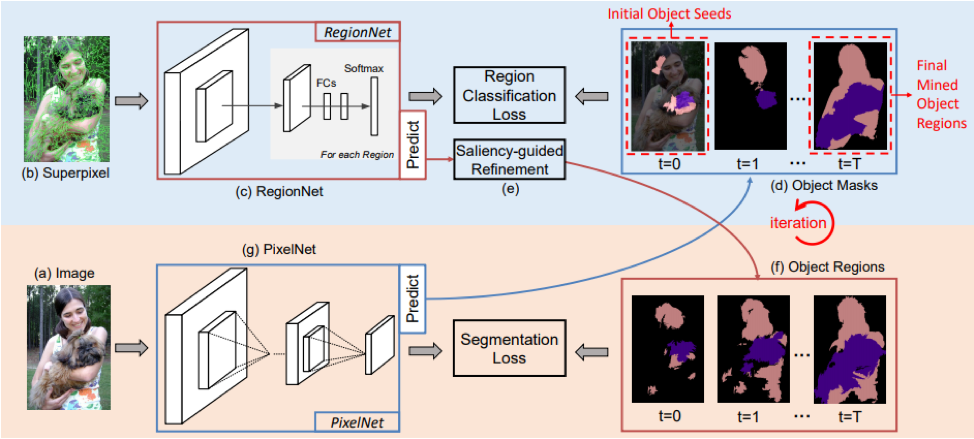
\includegraphics[width=\textwidth]{ref3_image}
	\caption{Pipeline of the proposed MCOF framework. At first (t=0), we mine common object features from initial object seeds. We segment (a) image into (b) superpixel regions and train the (c) region classification network RegionNet with the (d) initial object seeds. We then re-predict the training images regions with the trained RegionNet to get object regions. While the object regions may still only focus on discriminative regions of object, we address this by (e) saliency-guided refinement to get (f) refined object regions. The refined object regions are then used to train the (g) PixelNet. With the trained PixelNet, we re-predict the (d) segmentation masks of training images, are then used them as supervision to train the RegionNet, and the processes above are conducted iteratively. With the iterations, we can mine finer object regions and the PixelNet trained in the last iteration is used for inference. \cite{Wang2018WeaklySupervisedSS}}
	\label{fig:ref3}
\end{figure}

\paragraph{RegionNet}
Classification networks can produce initial localization of regions (hypothetically) containing significant common features about objects. After each training round (epoch), the refined object regions (output of PixelNet) are used as training data to predict object masks (new initial localization, higher accuracy).

\paragraph{PixelNet}
From these initial localizations outputted from RegionNet, common object features were mined. The object regions were expanded with mined features. 

\paragraph{Saliency-guide}
To segment non-discriminative regions, saliency maps are then considered under Bayesian framework to refine the object regions. 

\subsubsection{Experimental setup}

\paragraph{Data}
Pascal VOC 2012 dataset: 20 class objects + 1 background class. For the segmentation task, it contains 1464 training, 1449 validation and 1456 test images. They used augmented data of 10,582 images as training set.

\paragraph{Hardware}
Not mentioned!

\subsubsection{Results}
The MCOF framework outperformed previous state-of-the-art weakly-supervised semantic segmentation models by large margin. The performance metrics for comparison is mIOU (mean Intersection over Union of all 21 classes), and benchmark models included CCNN, EM-Adapt, MIL-sppxl, STC, DCSM, BFBP, AF-SS, SEC, CBTS and AE-PSL.

\paragraph{Conclusion}
The MCOF framework has two main advantages over previous approached. First, the iterative bottom-up and top-down framework tolerates inaccurate initial object localization. By iteratively mining common object features, the model can progressively produce segmentation masks with improving accuracy. Second, saliency-guided refinement method can allow for non-discriminative regions in initial localization, hence increase segmentation accuracy. This framework established new state-of-the-art performance.

\newpage

\bibliographystyle{unsrt}
\bibliography{ref}

\end{document}